\textbf{See the instruction for questions \inteval{\value{question}+1} to \inteval{\value{question}+2}.}

\begin{figure}[H]
    \centering
    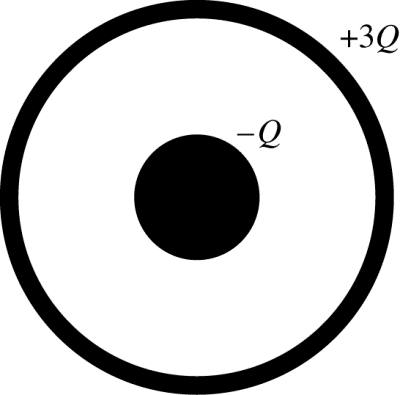
\includegraphics[scale=0.4]{images/img-013-020.png}
\end{figure}

A hollow conducting sphere is surrounded by a larger concentric spherical conducting shell, as shown above. The inner sphere has a net charge of $-Q$, and the outer sphere has a net charge of $+3 Q$.

% Multiple Choice Question 27
\begin{questions}\setcounter{question}{26}\question
What is the net charge on the inner surface of the spherical shell?

\begin{oneparchoices}
\choice $-Q$
\choice Zero
\choice $+Q$
\choice $+2Q$
\choice $+3Q$
\end{oneparchoices}\end{questions}

% Multiple Choice Question 28
\begin{questions}\setcounter{question}{27}\question
What is the net charge on the outer surface of the spherical shell?

\begin{oneparchoices}
\choice Zero
\choice $+Q$
\choice $+2Q$
\choice $+3Q$
\choice $+4Q$
\end{oneparchoices}\end{questions}

